\chapter{The Target Fan}
\label{target}
The target system within HELIOS consists of three main parts.  First, a mounting rail runs the length of the solenoid at the bottom of the vacuum chamber  (see Fig.~\ref{schematic} on p.~\pageref{schematic}).  This rail is an 80/20-brand 3.81\,cm square extruded aluminum T-slotted profile.  The mounting rail is attached to a mechanical feedthrough at the downstream end of the solenoid which allows the  rail to rotate under vacuum.  The second component of the target system is a support arm connected to the mounting rail by a linear bearing which allows for longitudinal motion of the assembly.   The final component of the target system is the modular target fan.

\section{Targets}
The original target fan design, shown on the left in Fig.~\ref{fan}, was milled out of a 6.35\,mm thick aluminum block.  Nine target positions are located along the outer edge of the fan at a radius of 43.50\,cm with each position separated by 4$^\circ$.  The spacing of the target positions is fixed by the width of a typical target frame.  With this geometry, the restricted rotation of a 3.81\,cm square support rail mounted at the bottom of the vacuum chamber limits the number of possible target positions to nine.

\begin{figure}%
\centering
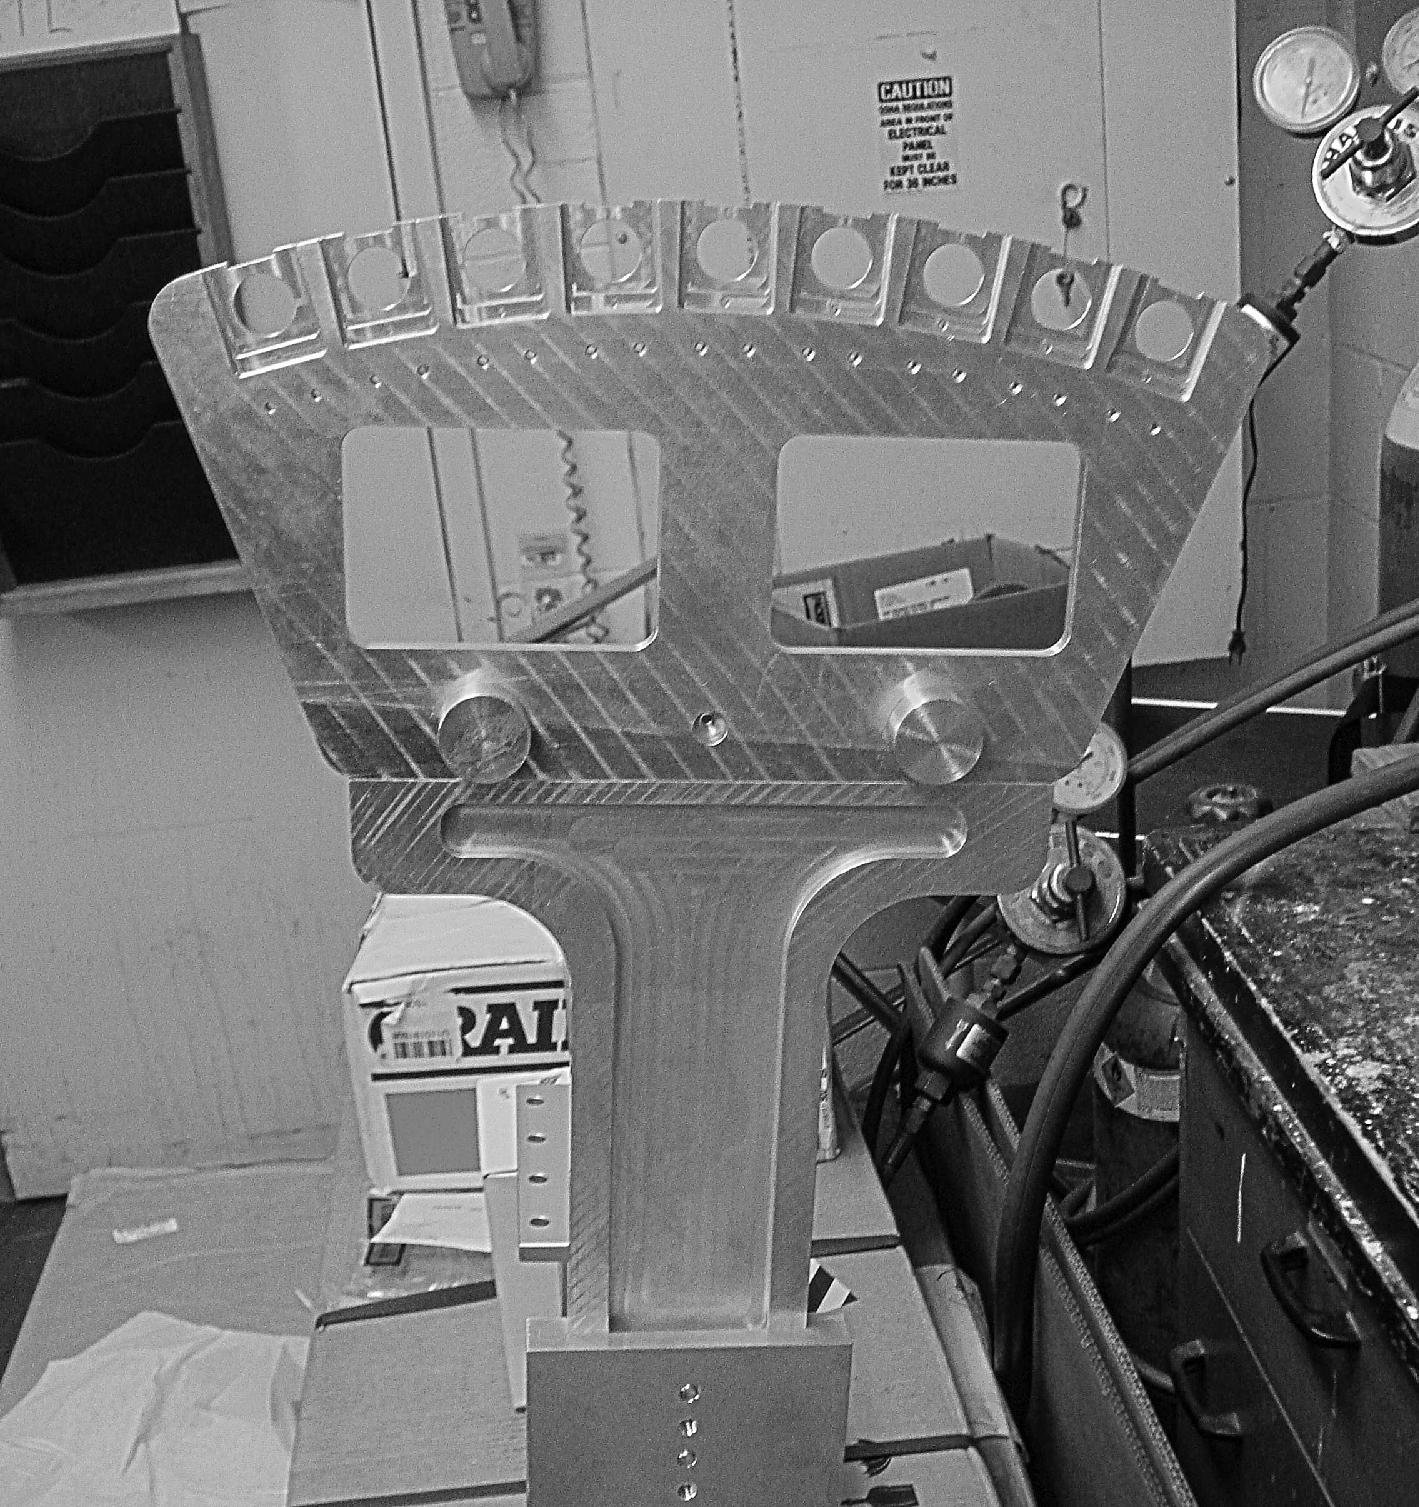
\includegraphics[width=.45\columnwidth,height=0.4\textheight,keepaspectratio]{DSC01459}~
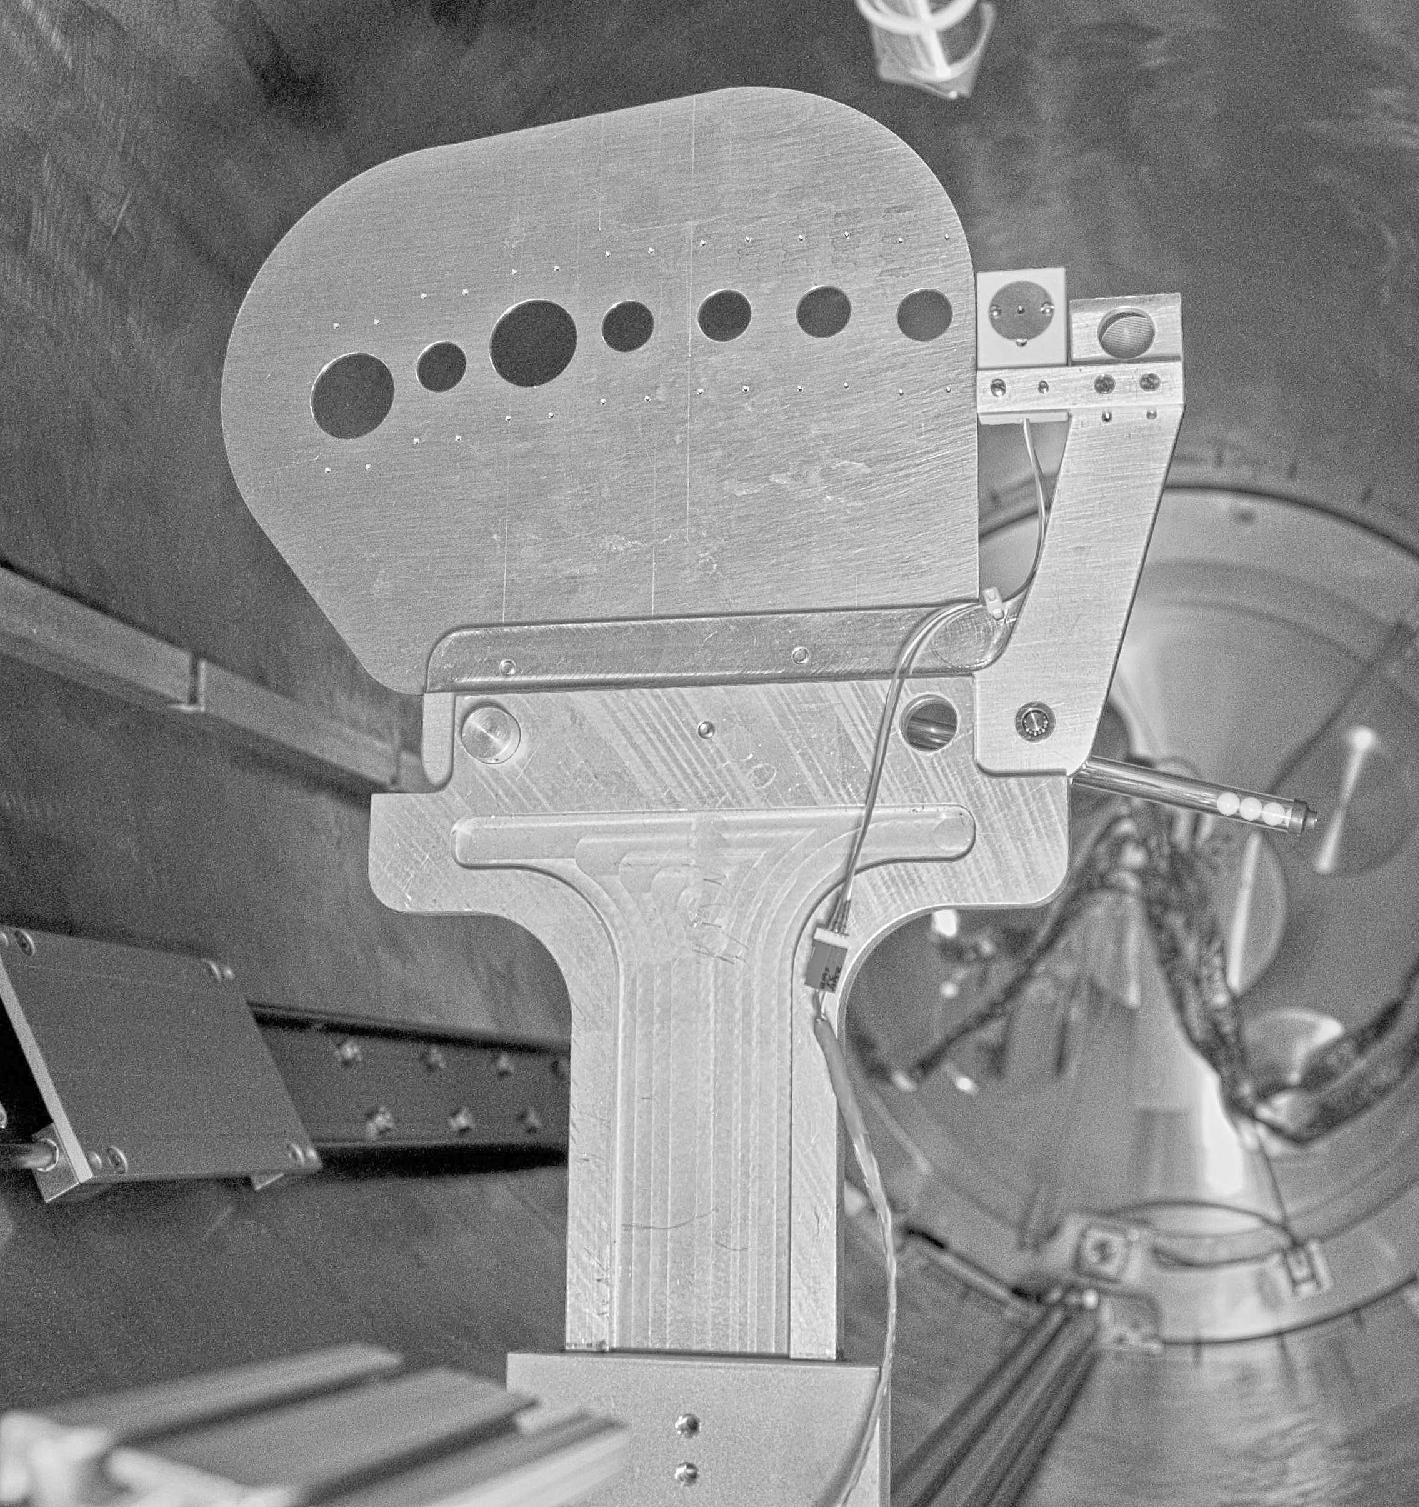
\includegraphics[width=.45\columnwidth,height=0.4\textheight,keepaspectratio]{_DSC3108}%
\caption[Two design iterations of the HELIOS target fan]{Two design iterations of the HELIOS target fan; (left) the Mark I design during assembly, and (right) the Mark II design installed in HELIOS.  The original designed featured a fan milled out of 6.35\,mm thick aluminum block.  The updated design is made from a piece of 1.5\,mm sheet metal.  Both designs feature nine target positions.}%
\label{fan}%
\end{figure}

In a typical experimental setup, four or five of the target positions are occupied by target foils.  For example, in a ($d$,$p$) reaction, a number of deuterated polyethylene (C$_2$D$_4$)$_n$ targets will be loaded into the target fan along with a carbon (foil for background measurements).  Various polyethylene foils may be installed for a range of target thicknesses or in case of breakage or damage. %
\subsection{Diagnostics}
In addition to target foils, the target fan can also hold a variety of diagnostic equipment including a radioactive decay source (typically $^{228}$Th or $^{148}$Gd-$^{244}$Cm) for detector calibration; a Faraday cup and collimator to measure the on-target beam current during tuning; and a silicon detector telescope in a $\Delta E$-$E$ configuration for beam-particle identification.  It has also been proposed to install a scintillating crystal for weak beam tuning.  This would require a high-sensitivity camera with a telescopic lens installed on one of the 16.51\,cm diameter feedthroughs.

\subsection{Acceptance}
One face of the target fan has 2.54\,mm recesses for mounting target frames---this side of the target frame is shown on the left-hand side of Fig.~\ref{fan}; the other face of the target fan has a 1.59\,cm aperture countersunk with a 90$^\circ$ chamfer at each target position.  This design is implicitly optimized for reactions with $K<1$ when the light ion ejectiles of interest are emitted in the rearward hemisphere.  With the target-foil side of the target fan facing the beam, ejectiles can be emitted at angles which are greater than $9.1^\circ$ from vertical.  The side of the target fan with countersunk apertures is intended to face downstream where the heavy ion reaction products are emitted in a narrow cone much smaller than the aperture chamfer.   However, if this side were to face the beam, the edge of the chamfer blocks orbits emitted at angles less than about $22^\circ$ from vertical.  This is consistent with the acceptance limit reported in Ref.~\cite{Lighthall_2010} and shown in Figs.~\ref{cezg_350} and \ref{double}.

To address the limited acceptance imposed by the original target fan, an updated design was made from a piece of 1.5\,mm sheet metal.  This design also features nine ``target'' positions, separated by $4^\circ$.  Two of the positions are dedicated to holding Faraday cup and a calibration source (see Fig.~\ref{fan}).  On the target-foil side of the updated fan, the acceptance limit has been lowered to $1.7^\circ$ from vertical.

\section{Positioning}
To align different target positions on the target fan with the beam axis, the target fan assembly is rotated about the axis of the support rail.  The longitudinal position of the target fan is adjusted by sliding the target assembly parallel to the beam axis %along the support rail
by means of a linear bearing.  Both of these adjustments can be made while the spectrometer is under vacuum.
\subsection{Translation}
\label{fantrans}
The target-to-array separation distance can be changed by moving the target fan as well as the detector array.  The linear bearing supporting the target fan moves along the mounting rail by means of a plastic chain drive which is controlled via a mechanical feedthrough. For the commissioning experiments, the position of the target fan was determined using a 2\,m aluminum ruler, measuring the distance between the support arm of the target fan and the flange face of the solenoid bore.  The support arm is milled out of a 1.27\,cm thick block of aluminum.  The interior surface of the support arm is milled down to a thickness of 0.32\,cm (see Fig.\ref{fan}).  This recessed face of the support arm is the reference face for measuring the position of the target fan.  A measurement of 1175\,mm was defined as the center of the magnet ($z=0$).

Subsequent measurements utilized a AccuRange model AR1000 Laser Distance Sensor.  The laser range finder uses standard RS232 serial interface to communicated computer.  A simple LabVIEW\texttrademark{} ``virtual instrument'' (VI) was created to monitor the output from the laser.  Initially, the range finder was mounted inside the vacuum chamber on the rail supporting the target fan.  However, in this configuration, the laser system fails to operate at a solenoid current of 82\,A, corresponding to a central field of 0.45\,T.  The laser was then moved to the beam line stand upstream of the solenoid, at a distance of 2.5\,m from the solenoid where the on-axis fringe field is less than 130\,G.  A small anti-reflective glass port was installed on one of the 16.51\,cm diameter feedthroughs.

Range measurements are made by rotating the target fan into the path of the laser, so that the laser hits the reference plane of the target fan support (now, on the upstream side of the target fan).  The position of the target fan was calibrated by zeroing the range finder reading with the target fan at the $z=0$ position described above.  The range finder has a stated accuracy of $\pm 2.5$\,mm.  A reflecting arm has also been attached to the detector array support which can be rotated into the path of the laser beam for distance measurements.

\subsection{Rotation}
The target fan can rotate over a range of about $\pm 18^\circ$ from vertical.  The rotation of the target fan is controlled by a Danaher Motion series CTP3 stepper motor.   The motor is connected to the mechanical feedthrough of the target fan mounting rail by a worm gear which is driven by a 1\,m drive shaft.  The target drive motor is located about 1.5\,m away from the solenoid axis to reduce the magnetic field in which the motor operates. The worm gear assembly and target drive is shown in Fig.~\ref{worm_gear}.

\begin{figure}%
\centering
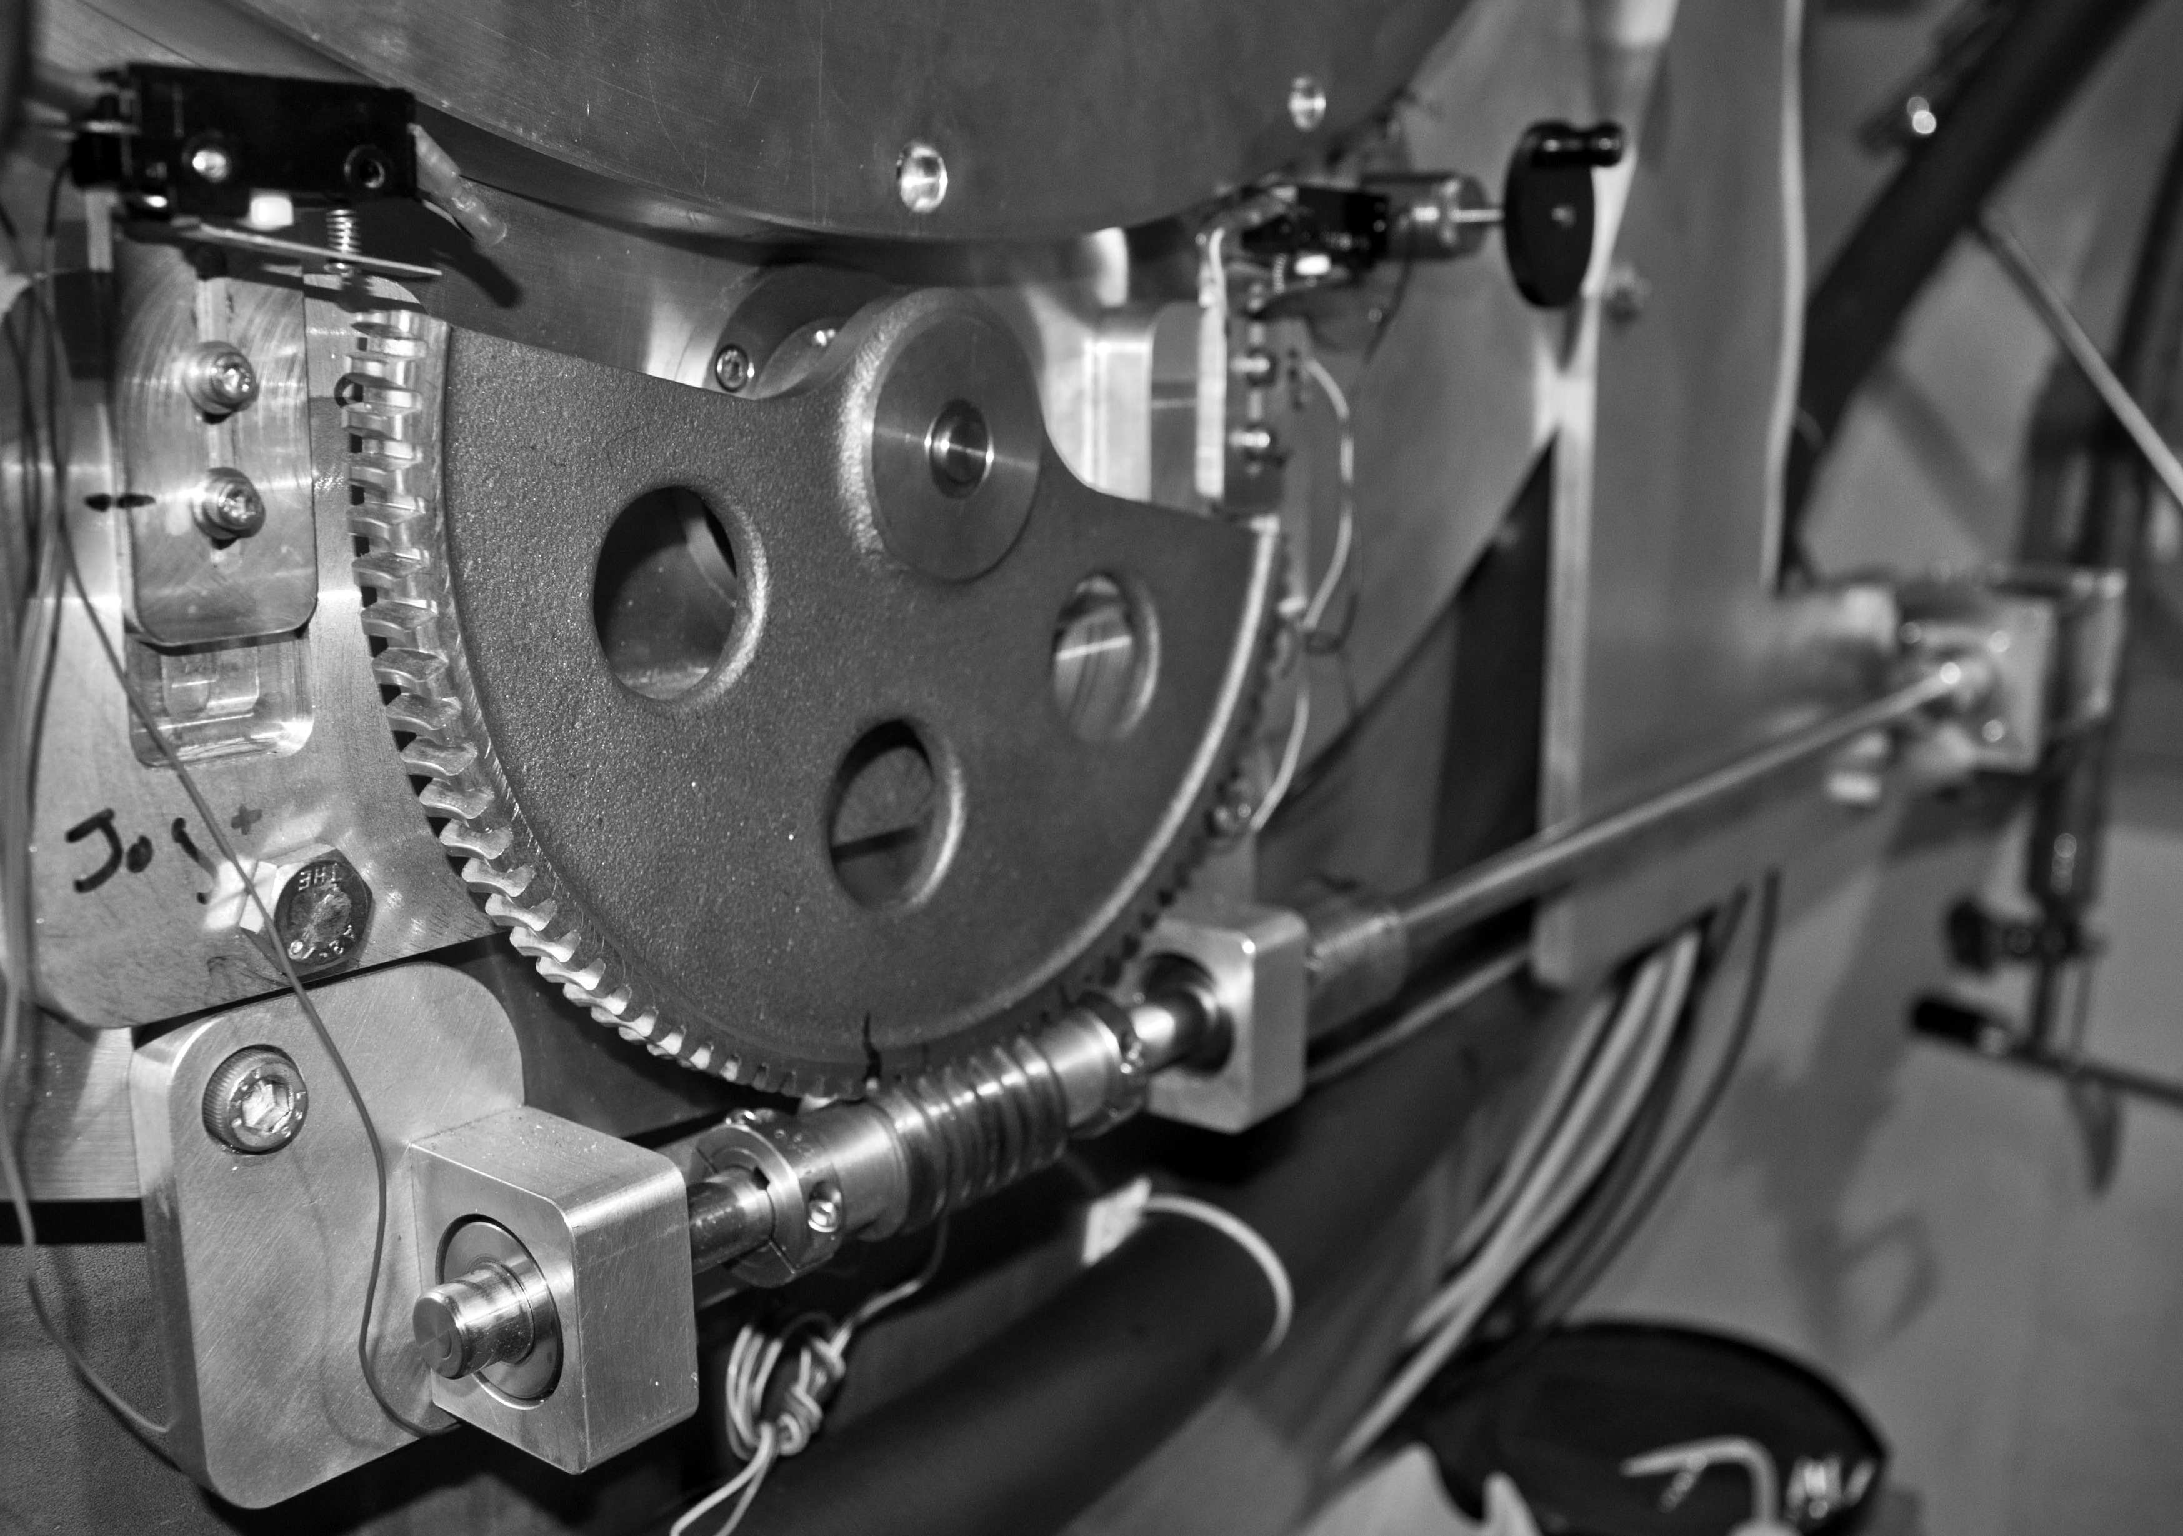
\includegraphics[width=\columnwidth,height=0.4\textheight,keepaspectratio]{_DSC3111}%
\caption[Detail of the target drive located on the downstream end of the HELIOS solenoid]{Detail of the target drive located on the downstream end of the HELIOS solenoid.  In the foreground, the worm gear connects to a mechanical feedthrough at the lowest point of the vacuum chamber adapter flange.  Extending into the background is a 1\,m drive shaft connecting the worm gear to the stepper motor.}%
\label{worm_gear}%
\end{figure}

The stepper motor is controlled with a National Instruments model PCI-7330 stepper motor controller and an auxiliary manual control interface.   The software package NI-Motion\texttrademark{} which accompanied the stepper motor controller provided programing modules which allows basic control of the stepper motor such as \textit{move} and \textit{stop}.  A high-level user interface, shown in Fig.~\ref{labview}, is built upon these commands.  The electronic noise produced by the stepper motor power supply interferes with the detector array preamplifiers.  Therefore, the stepper motor is de-energized during data acquisition.

\begin{figure}[t]%
\centering
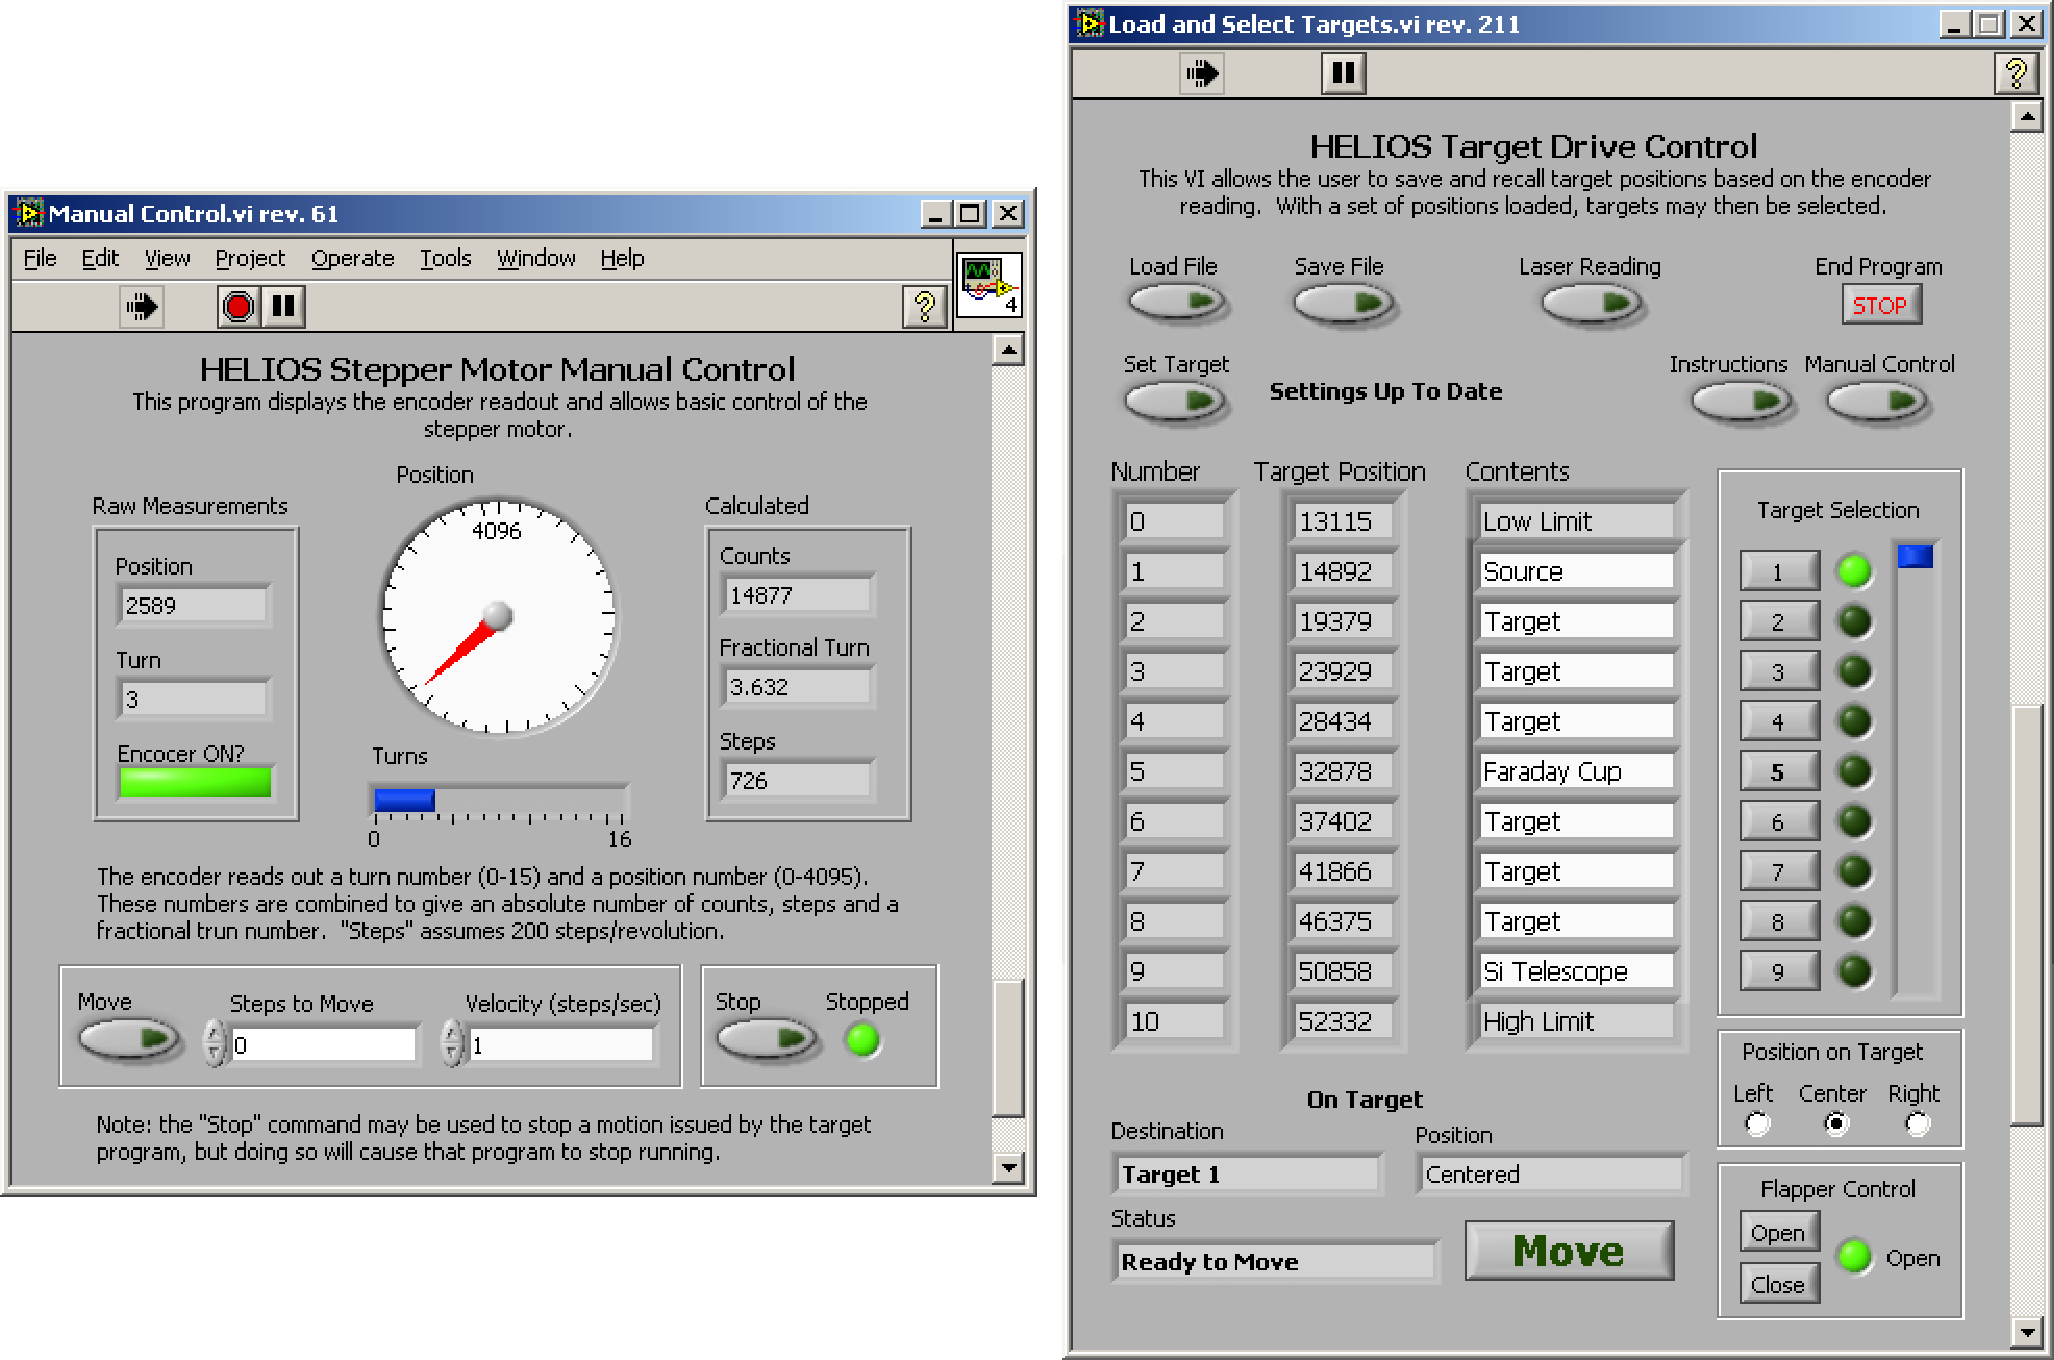
\includegraphics[width=\textwidth,height=0.5\textheight,keepaspectratio]{target_drive}%
\caption[Screenshots of the program using LabVIEW\texttrademark{} which controls the rotation of the target drive]{Screenshots of the program using LabVIEW\texttrademark{} which controls the rotation of the target drive  (left) The \texttt{Manual Control} VI displays the output of the encoder and allows simple control of the stepper motor.  (right) The \texttt{Load and Select Targets} VI allows the user to store and recall target positions based on the encoder readings.  Once position settings are loaded, the user may move the target fan to a specific target by selecting the desired target within the program and issuing the \textit{move} command.  The target drive program then automatically moves the target fan to the correct position using the encoder readings for feedback and adjusting for backlash, if necessary.  The program provides a reproducibility (precision) of $<0.5$\,mm.}%
\label{labview}%
\end{figure}

The stepper motor has a rear-end drift shaft which is connected to a BEI Industrial Encoders model HMT25 encoder to monitor the position of the target fan.  Three bytes are read out from the encoder.  First, a 12-bit integer (output over two bytes) indicates the position of the encoder within a given turn, yielding 4096 digits per turn.  This is followed by a 4-bit integer (output over one byte), giving the turn number (0 to 15).  This corresponds to an encoding resolution of 4096 bits/revolution or 0.088$^\circ$ (1.5\,mrad) over 16 rotations.

The stepper motor is capable of moving in increments of 1.8$^\circ$ (200 steps/revolution).  Therefore, one step of the stepper motor---an interval of 1.8$^\circ$---corresponds to 20 or 21 (20.48) encoder digits.  As a result, the stepper motor must be operated using live feedback from the encoder.  For example, given a specific position that needs to be reproduced, the stepper motor is adjusted until the encoder reads the desired position within $\pm 10$ encoder digits.  Furthermore, to account for the finite spacing between the teeth of the worm and the worm gear (``backlash''), all aligning motions must be performed with the desired position approached from the same direction.  The target drive program, shown in Fig.~\ref{labview}, accounts for both backlash and the precision of the stepper motor automatically.

The a worm gear which transfers the rotation of the stepper motor to the mounting rail has a ratio of 1:100.   With the target foils rotating on a radius of 43.50\,cm, a rotation increment of 1.8$^\circ$ at the stepper motor corresponds to a target rotation of 0.018$^\circ$ and a (theoretical) arc length precision of 0.14\,mm.  However, the effective arc length precision is about 0.5\,mm.  Each target foil is ``sighted in'' using an alignment telescope and the manual control interface.  The encoder positions of target foil are then saved in the automated target drive controller program (see Fig.~\ref{labview}).  Once a reference set of target foil position has been stored---since the spacing of the target foils is fixed---the position of the entire target fan assembly can be calibrated by sighting in a single target.

\section{Further Designs}
\subsection{Luminosity Monitor}
In order to make absolute cross section measurements, a precise determination of both the beam current and the target thickness must be made.  Due to the complex nature of the accelerator system, fluctuations in beam current are a normal part of operation.  In addition, any given target foil will have an inherent uncertainty in its thickness as well as possible variations in thickness.  Furthermore, depending on the beam intensity, the isotopic content of the foil may degrade significantly during the course of an experiment.

\begin{figure*}%
\centering
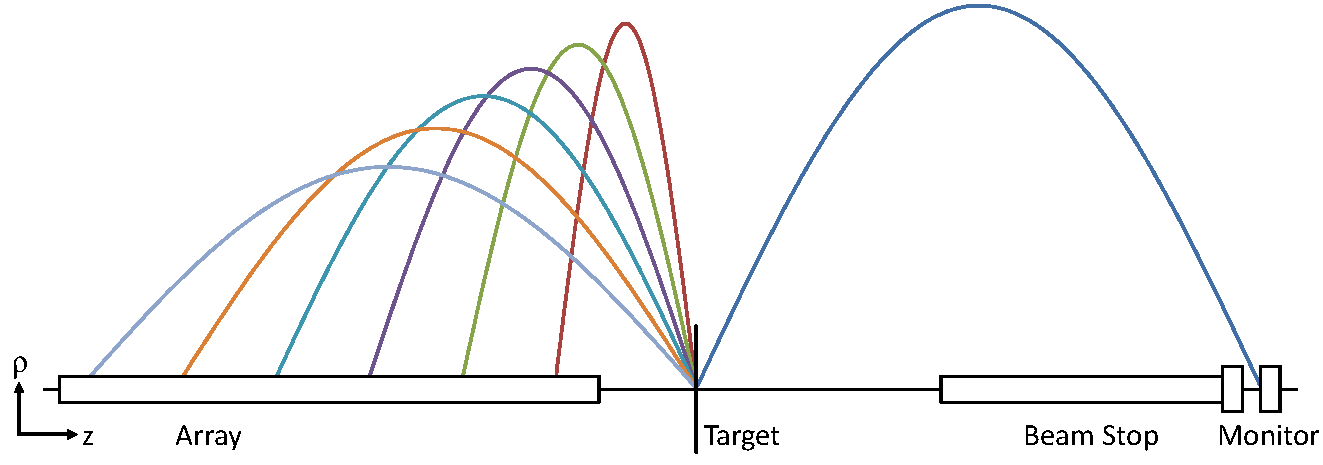
\includegraphics[width=\textwidth,height=0.4\textheight,keepaspectratio]{lumin}%
\caption[Illustration of the luminosity monitor design]{Illustration of the luminosity monitor design.  Calculated trajectories for 5\,\AMeV $^{136}$Xe on a deuterium target with $\mathscr{B}_0=2.0$\,T.  In the rearward hemisphere, protons from the ground-state transition of the ($d$,$p$) reaction intercept the array.  The plotted trajectories were calculated such that each trajectory intercepts the center of a detector element for a target-array setting of $\Delta z = 64$\,mm.  In the upstream hemisphere elastically scattered deuterons intercept the luminosity monitor located at $z=+360$\,mm, relative to the target.  The unreacted beam and beam-like reaction products are stopped in a Faraday cup which includes a backscattering baffle.  Adapted from Ref.~\cite{Kay_2010HID}.}%
\label{luminos}%
\end{figure*}

To monitor the isotopic content of the target foil and the incident beam current, the ``luminosity monitor'' illustrated in Fig.~\ref{luminos} is used~\cite{Kay_2010APS}.  In the downstream configuration shown in the figure, the beam passes through the silicon detector array and intercepts the target foil in the normal fashion.  The beam and beam-like heavy recoils are stopped in a Faraday cup which is at the end of a tube to block backscattered particles from being detected by the array.  The Faraday cup monitors the beam current which can be used to determine the differential cross section.  The luminosity $L$ is related to the differential cross section $d\sigma/d\Omega$ by the equation
\begin{equation}
\frac{d\sigma}{d\Omega}=\frac{1}{L}\frac{d^2 N}{d\Omega dt}
\label{luminosity}
\end{equation}
where $N$ is the number of interactions, determined by the count rate in the detector array; and $d\Omega$ is the differential solid angle (determined from geometry, see \S\,\ref{accept}).  

Past the beam stop, a surface barrier silicon detector measures elastically scattered target ions.  For example, with a deuterated polyethylene target, this detector is used to monitor deuterons from ($d$,$d$).  In the arrangement shown in Fig.~\ref{luminos}, the detector is placed 360\,mm upstream from the target to measure 3.5\,MeV elastically scattered deuterons, corresponding to a scattering angle of $\theta_\mathrm{lab}=72.5^\circ$.  In the Rutherford energy regime, the count rate in the monitor detector can be compared to previously-determined Rutherford scattering cross sections.  The ratio of these cross sections can be used to scale the differential cross section measured in the detector array to calculate an absolute cross section.  At energies above the threshold for Rutherford scattering, the rate in the surface barrier detector can be used to monitor the isotopic content of the target.

Although not specifically a target, the luminosity monitor was originally installed on the rotating support rail of the target fan.  In this configuration, the luminosity monitor rotated with the target fan and could only be used in conjunction with one target position.  Later designs utilized auxiliary support rails running the length of the solenoid.  With the luminosity monitor mounted independently of the target fan, various target positions could be utilized.

\subsection{Gas Cell}
As of this writing, construction is under way of a cryogenic  gas cell target which can be put in place of the HELIOS target fan.  The cryogenic target fan features one gas cell and six positions for solid target foils and diagnostics.  An engineering schematic is shown in Fig.~\ref{gas_fan}.  The length (thickness) of the gas cell is about 1.5\,mm and has an opening angle of $144^\circ$.  The gas cell is a redesign of a similar gas cell which was used in a previous measurement at Argonne~\cite{Sonzogni_2000}.  As of this writing, 2--4 days of beam time have been approved to test the gas cell in HELIOS with the $^{25}$Al($^3$He,$d$)$^{26}$Si reaction. 

\begin{figure}[hb]%
\centering
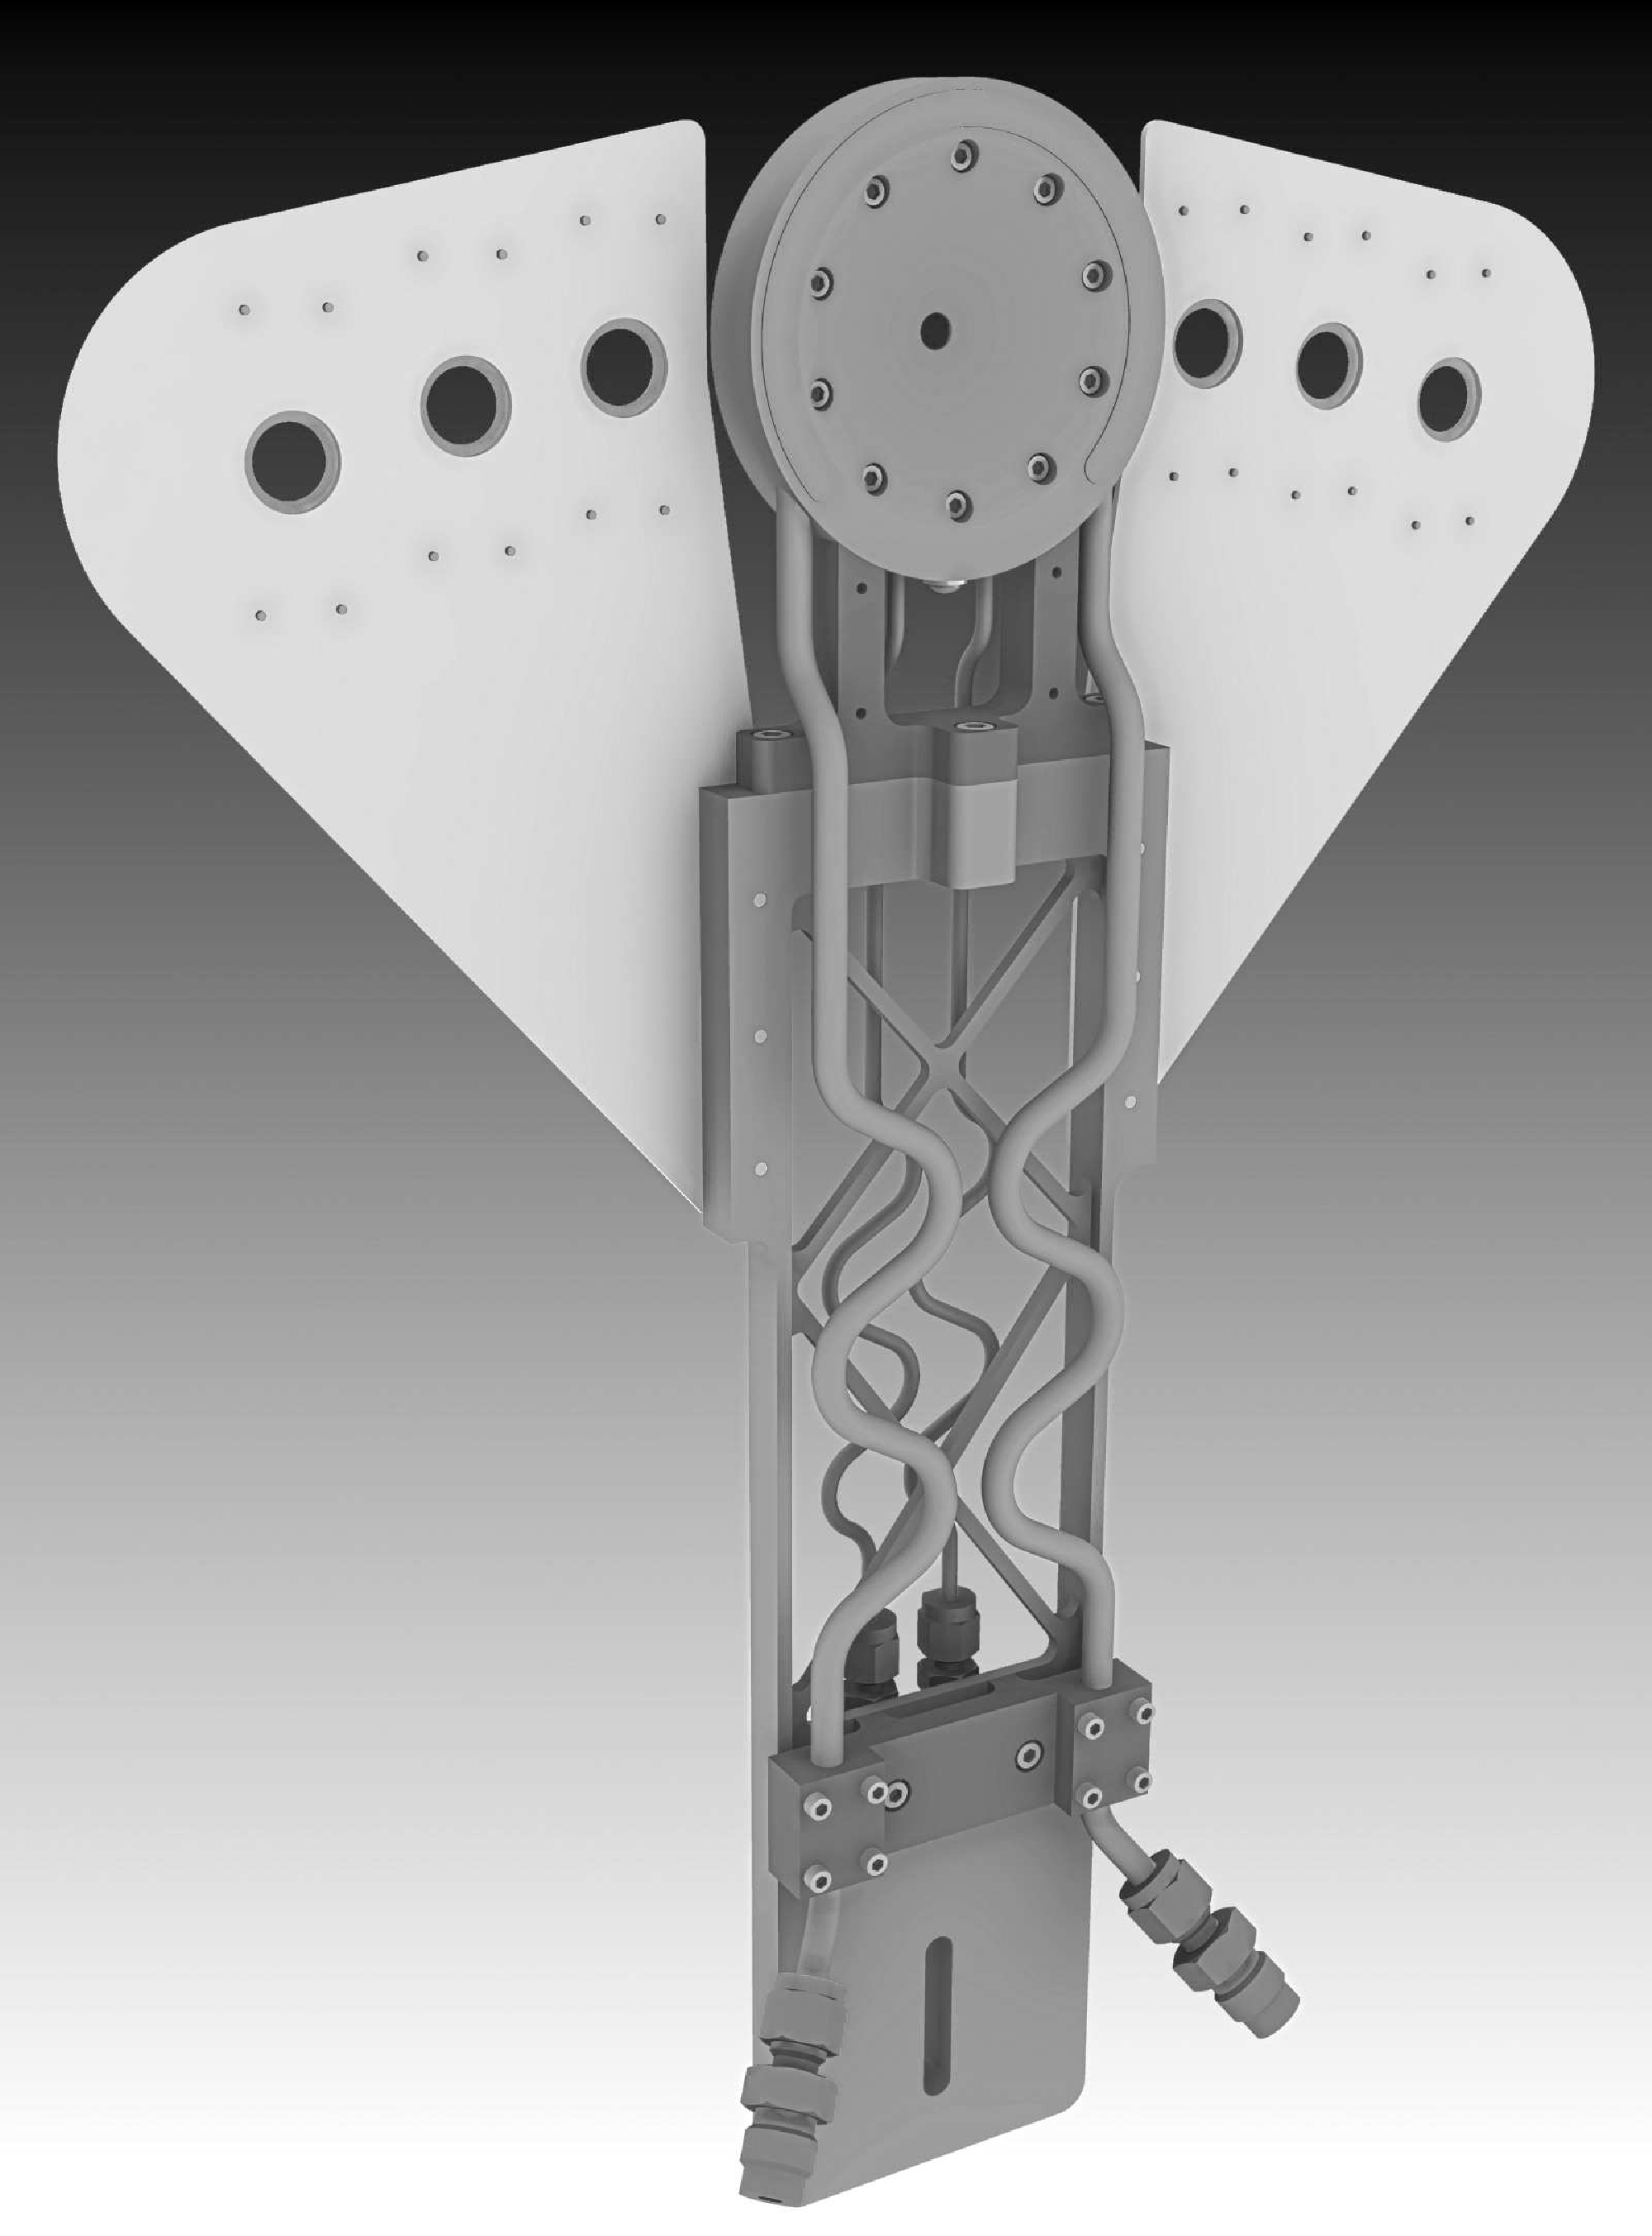
\includegraphics[width=\columnwidth,height=0.3\textheight,keepaspectratio]{HELIOS_Cryo_Target}%
\caption[HELIOS cryogenic gas cell target fan]{HELIOS cryogenic gas cell target fan. Designed and rendering by B.~J.\ DiGiovine.}%
\label{gas_fan}%
\end{figure}